\chapter{Programmazione Lineare Intera}
Un generico problema di programmazione lineare intera (detto PLI) è

\[\min c^T x \quad Ax = b \quad x \geq 0 \quad x \text{ INTERO}.\]

La regione ammissibile di un problema di PLI non è più convessa.
Mettendo a confronto la regione ammissibile di PLI (che chiameremo X) con la corrispettiva regione ammissibile del problema PL (che
chiameremo P) senza vincolo di intero la regione ammissibile risulta sostanzialmente che X = P intersecato $Z^n$ (non più convessa).
\begin{figure}[H]
    \centering
    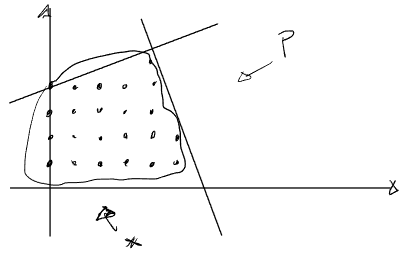
\includegraphics[width=0.5\linewidth]{Images/programmazione_lineare_continua/regione_ammissibile_x_p.png}
\end{figure}
Sappiamo per certo che:
\[\min c^T x \quad \in P \leq \min c^Tx \quad \in X\]
Per cui il valore ottimo del problema continuo è un lower bound rispetto al valore ottimo del problema intero.

Si dice \textbf{rilassamento continuo/lineare} il problema di PL ottenuto dal problema PLI eliminando il vincolo di interezza. Quindi il valore ottimo della funzione obiettivo del rilassamento lineare è minore o uguale del valore ottimo della funzione obiettivo del problema intero.
Se il rilassamento dà una soluzione ottima intera è anche soluzione ottima di PLI.

Si osserva che se la funzione ottima di RL non è intera, la sua approssimazione per eccesso o per difetto non dà la soluzione ottima intera.
Dato l'insieme ammissibile di PLI esistono infiniti poliedri continui che lo contengono per cui:
\begin{figure}[H]
    \centering
    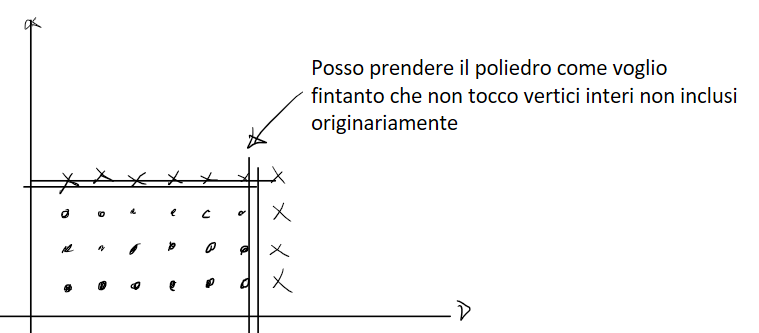
\includegraphics[width=0.5\linewidth]{Images/programmazione_lineare_continua/problema_chill.png}
\end{figure}
Il miglior poliedro è dato dalla combinazione convessa dei punti interi e viene detto \textbf{poliedro convessificato}.Per cui varrà che:
\[\min c^T x \quad \in X = \min c^T x \quad \in conv(X)\]

Per cui, varrà che tutti i vertici di $conv(x)$ saranno interi.
\section{Problemi Ideali}
I problemi ideali sono dei problemi continui la cui soluzione è intera. Questi hanno una struttura particolare della matrice A.\\ 
Una matrice A di tipo m x n si dice \textbf{unimodulare} se ogni sottomatrice m x m ha determinante o -1 o 0 oppure 1. \\
\textbf{Teorema}\\
Dato il poliedro $P = \{ x \in R^N : Ax = b, x \geq 0 \}$, se A è unimodulare e b ha componenti intere, allora P ha vertici interi.
Dunque, se abbiamo un problema di PLI con $X = \{ x \in R^N, Ax = b, x \geq 0, x \text{ intero}\}$  con A unimodulare e B con solo componenti intere, possiamo risolvere il rilassamento lineare e trovare una soluzione intera.\\
Una matrice A $m \times n$ è \textbf{totalmente unimodulare} (TU) se ogni sottomatrice quadrata $p \times p$ di ogni ordine ha determinante che vale -1,0,1.
Di conseguenza una matrice totalmente unimodulare ha solo elementi -1,0,1 per cui \textbf{ha sempre soluzione intera}\\

Sia A una matrice con elementi -1, 0, 1 e con al massimo 2 elementi diversi da o in ogni colonna, A è totalmente unimodulare se e solo se esiste una partizione $R_1$ e $R_2$ delle righe in modo che nelle colonne con 2 elementi diversi da 0, se gli \textbf{elementi sono concordi appartengono a partizioni diverse, se sono discordi appartengono alla stessa partizione}.
Allo stesso modo, Sia A una matrice $m \times n$ con elementi 0,1,-1 e tale che in ogni colonna ci sono al massimo due elementi diversi da 0. Se in tali colonne la \textbf{somma degli elementi è 0}, allora A è totalmente unimodulare.
\subsection{Problema del Flusso di Costo Minimo}
Consideriamo una rete $G=(N,A)$, a ogni arco $(i,j)$ associamo un costo $c_{ij}$ e a ogni nodo $i$ associamo un peso $b_i$.
\begin{enumerate}
    \item Se $b_i > 0$, allora è un \textbf{nodo sorgente}.
    \item Se $b_i < 0$, allora è un \textbf{nodo destinazione}.
    \item Se $b_i = 0$, allora è un \textbf{nodo di transito}.
\end{enumerate}
Dato questo grafo, vogliamo determinare il flusso $X=(x_{ij}) : i,j \in A$, cioè il flusso che scorre lungo la rete in modo da minimizzare il costo e soddisfare il vincolo di bilancio, cioè: 
\[\forall i \quad \text{flusso uscente - flusso entrante} = b_i\]
In formule: 
\begin{align*}
    &\min (\sum_{ij \in A} c_{ij}x_{ij})\quad \text{ Costo totale}\\
    &\sum_{j : j \in A} x_{ij} - \sum_{j: j \in} x_{j, i} > b_i \quad \forall i \in N \quad \text{ Flusso in uscita - flusso in entrata}
\end{align*}

Vediamone un esempio:
\begin{figure}[H]
    \centering
    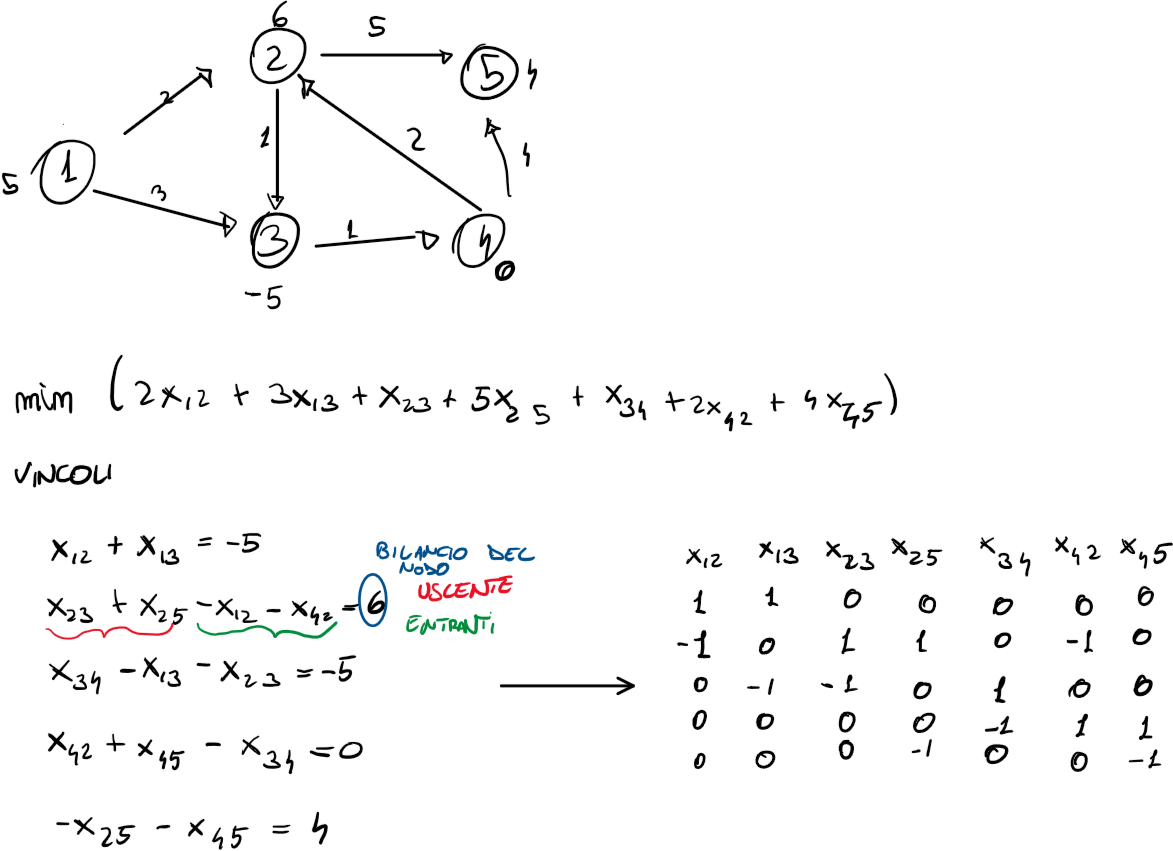
\includegraphics[width=0.8\linewidth]{Images/programmazione_lineare_continua/problema_del_flusso.png}
\end{figure}
Inquadriamolo meglio facendo corrispondere a ogni riga una nodo e a ogni colonna un arco. Vediamo che ci sarà 1 se esiste l'arco ed è uscente per il nodo in quella riga, 0 se l'arco non tocca il nodo nella riga, -1 se l'arco esiste ed è entrante nel nodo corrispondente alla riga.
\begin{figure}[H]
    \centering
    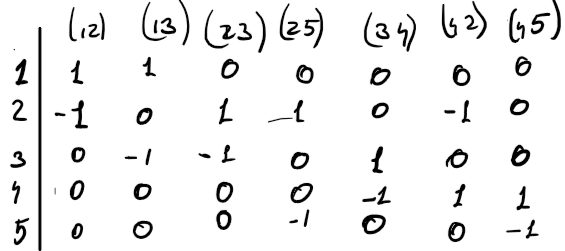
\includegraphics[width=0.5\linewidth]{Images/programmazione_lineare_continua/tabella_nodi_archi.png}
\end{figure}

\section{Metodo dei tagli di Gomory}
Questo metodo si basa sull'idea di risolvere una successione di rilassamenti lineari fino a trovare una soluzione intera. Lo schema generale prevede questo:
\begin{enumerate}
    \item Si risolve il rilassamento lineare. Se si trova una soluzione intera, allora ci fermiamo.
    \item Si introduce un nuovo vincolo che corrisponderà al \textbf{taglio}.
    \item Si risolve il nuovo rilassamento lineare.
\end{enumerate}
Possiamo immaginare un taglio in questo modo:
\begin{figure}[H]
    \centering
    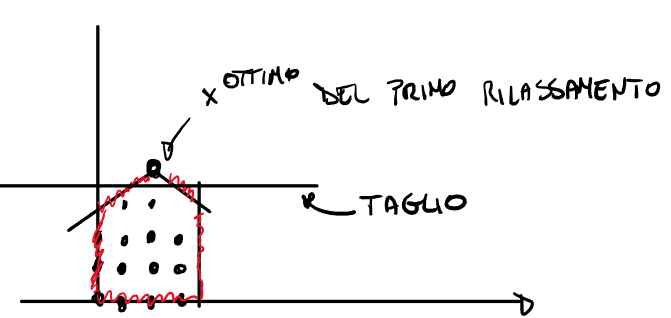
\includegraphics[width=0.5\linewidth]{Images/programmazione_lineare_continua/taglio_gomory.png}
\end{figure}
Diamo alcune definizioni prima di andare avanti.
Si dice disuguaglianza valida un vincolo soddisfatto da tutti i punti ammissibili interi. Quindi:
\[min c^T x \quad Ax = b \quad x \geq 0 \quad x \in N \]
Indichiamo con X la regione ammissibile e, dunque, una disuguaglianza valida sarà: $a^Tx \leq a_0 \quad \forall x \in X$
Diremo, quindi, che un taglio è una disuguaglianza valida per X che non è soddisfatta dalla soluzione ottima frazionaria del rilassamento lineare $x^{ott}_{RL}$.
\subsection{Applicazione dei tagli}
Supponiamo di aver risolto il rilassamento lineare con il metodo del simplesso e di aver ottenuto la seguente tabella con $\beta_r$ frazionario:
\begin{figure}[H]
    \centering
    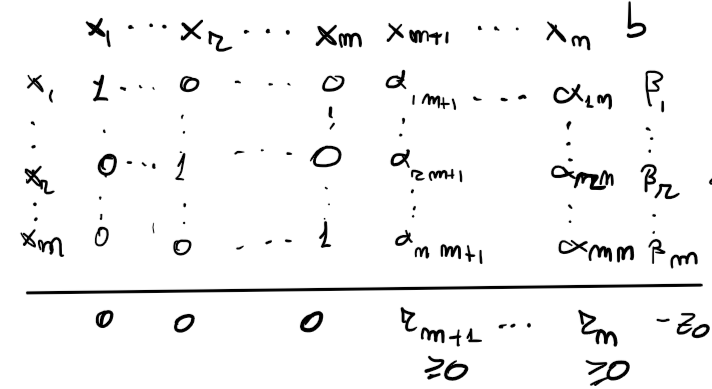
\includegraphics[width=0.5\linewidth]{Images/programmazione_lineare_continua/tabella_finale_simplesso_RL.png}
\end{figure}

Da questa tabella, segue che:
\begin{equation}
    \tag{1}
    x_r+\alpha_{r m+1} x_{r m+1} + \dots \alpha_{rn}x_n=\beta_r
\end{equation}
Possiamo arrotondare tutti gli $\alpha$ per difetto e scrivere:
\begin{equation}
    \tag{2}
    x_r+\lfloor \alpha_{r m+1}\rfloor x_{r m+1} + \dots \lfloor \alpha_{rn}\rfloor x_n=\lfloor \beta_r \rfloor
\end{equation}

A questo punto il taglio sarà (1)-(2), cioè:
\[(\alpha_{rm+1}-\lfloor \alpha_{rm+1} \rfloor ) x_{m+1}+ \dots +(\alpha_{rn}-\lfloor \alpha_{rn} \rfloor ) x_{n}-x_{n+1}=\beta_r - \lfloor \beta_r \rfloor\]

Fatto ciò, per evitare di perdere la base, moltiplichiamo ciò per -1: 
\[(\lfloor \alpha_{rm+1} \rfloor - \alpha_{rm+1} ) x_{m+1}+ \dots +(\lfloor \alpha_{rn} \rfloor - \alpha_{rn} ) x_{n}+x_{n+1}= \lfloor \beta_r \rfloor - \beta_r\]

Finito ciò, possiamo continuare con il simplesso duale poiché avremo che nella riga $r-esima$ abbiamo il termine noto che sarà certamente $<0$. Si nota che alla tabella abbiamo aggiunto una riga e una colonna.
Possiamo anche vederne un esempio:
\begin{figure}[H]
    \centering
    
\includegraphics[width=1\linewidth]{Images/programmazione_lineare_continua/esempio_tagli_gomory/1.png}
\end{figure}
\begin{figure}[H]
    \centering
    
\includegraphics[width=1\linewidth]{Images/programmazione_lineare_continua/esempio_tagli_gomory/2.png}
\end{figure}
\begin{figure}[H]
    \centering
    
\includegraphics[width=1\linewidth]{Images/programmazione_lineare_continua/esempio_tagli_gomory/3.png}
\end{figure}
\section{Metodo del Branch and Bound}
Questo metodo si  basa sull'idea di partizionare in modo ricorsivo la regione ammissibile del rilassamento lineare. Si risolvono, quindi, dei sottoproblemi le cui regioni ammissibili vengono, a loro volta, partizionate. Si terrà traccia dei problemi mediante un albero.
Il metodo individua le \textbf{regioni promettenti} sulle quali ricercare l'ottimo, e le regioni nelle quali non effettuare la ricerca dell'ottimo.\\
Troveremo due operazioni:
\begin{enumerate}
    \item \textbf{Bounding:} la risoluzione dei sottoproblemi continui fornisce un lower-bound per il valore ottimo della funzione obiettivo del problema di programmazione lineare intero. Si nota che si possono ottenere dei lower-bound anche con altri tipi di rilassamenti oltre a quello lineare.
    \item \textbf{Branching:} è l'operazione che permette di partizionare la regione ammissibile dei rilassamenti lineari. 
\end{enumerate}


Consideriamo un generico problema di PLI:
\[\min c^T x \quad Ax \geq b \quad x = 0 \quad x \in N\]
Tipicamente, si costruisce il rilassamento lineare:
\[\min c^T x \quad Ax \geq b \quad x \geq 0 \]
D'ora in avanti segnaleremo il RL come $P_0$ poiché sarà il primo nodo da cui partiremo per risolvere il problema. Sia $x^0$ la soluzione ottima di $P_0$ e supponiamo che la componente $x^0_h$ sia frazionaria. 
\begin{figure}[H]
    \centering
    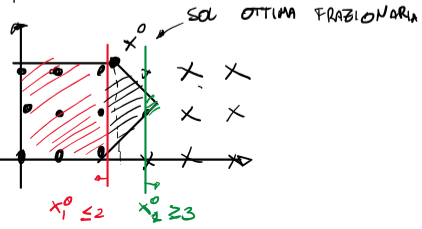
\includegraphics[width=0.5\linewidth]{Images/programmazione_lineare_continua/branch_bound.png}
\end{figure}
A questo, come vediamo in figura, possiamo aggiungere un vincolo di $\leq$ (in rosso) o di $\geq$ (in verde) facendo il floor o il ceeling della variabile la cui componente è frazionaria. Così, dividiamo il grafico in tre parti, due di queste saranno soggette a una ricerca dell'ottimo mentre l'altra verrà esclusa poiché non contiene soluzioni intere. Immaginiamo quindi un albero di ricorsione di problemi, gestito a questo modo:
\begin{figure}[H]
    \centering
    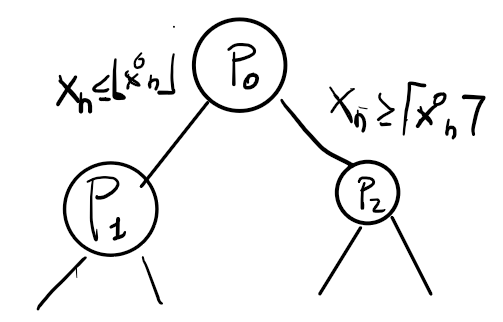
\includegraphics[width=0.5\linewidth]{Images/programmazione_lineare_continua/albero_sottoproblemi.png}
\end{figure}
La ramificazione è detta operazione di branching, la variabile $x_h$ è detta variabile di branch. Risulta che il lower-bound dato da $P_0$ è sempre minore o uguale del lower-bound fornito dai suoi figli.
\subsection{Criteri di Potatura}
I criteri di potatura ci dicono quando smettere di visitare un nodo seguendo delle specifiche regole:
\begin{enumerate}
    \item Un nodo si chiude se dà una soluzione intera.
    \item Un nodo si chiude per inammissibilità se il vincolo di branch è in contrasto con i vincoli precedenti generando così una regione ammissibile vuota.
    \item Un nodo si chiude per \textbf{bounding} quando la soluzione di un sottoproblema è frazionaria e dà un valore della funzione obiettivo peggiore del valore ottimo corrente. Non ci fermiamo alla prima soluzione intera che troviamo ma abbiamo bisogno di seguire i criteri di potatura.
\end{enumerate}
\subsection{Criteri di Visita}
Allo stesso modo, abbiamo alcuni criteri detti di visita che stabiliscono un ordine nei sottoproblemi da visitare. Questi sono:
\begin{enumerate}
    \item \textbf{Visita in profondità:} si esplora il primo figlio di ogni nodo fino a quando non si deve risalire al primo nodo aperto. Si minimizza il numero di nodi aperti e i requisiti di memoria, di contro si visitano tanti nodi.
    \item \textbf{Visita per best-bound:} si risolve prima il problema con il lower-bound migliore. Si risolve P0, P1 e P2, si confrontano i lower-bound di tutti i problemi risolti e si esplora il nodo migliore. A ogni problema risolto si confronta il lower-bound tra tutti i problemi aperti. Si visitano minimizzano i nodi esplorati ma si tengono più problemi aperti da visitare.
    \item \textbf{Metodo ibrido:} si fissa il numero massimo di problemi aperti da esplorare e si visita per best-bound. Raggiunto il limite si procede con la visita in profondità.
\end{enumerate}

Vediamo subito un esempio di come applicare questo metodo seguendo il criterio di visita best-bound.
\begin{figure}[H]
    \centering
    
\includegraphics[width=1\linewidth]{Images/programmazione_lineare_continua/esempio_branch_bound/1.png}
\end{figure}
A questo punto, scegliamo $x_1$ come variabile di branch e generiamo $P_1, P_2$
\begin{figure}[H]
    \centering
    
\includegraphics[width=1\linewidth]{Images/programmazione_lineare_continua/esempio_branch_bound/2.png}
\end{figure}
Cerchiamo di proseguire quindi da $P_2$ generando $P_3, P_4$, scoprendo però che $P_4$ genera un problema inammissibile, quindi si chiude il nodo.
\begin{figure}[H]
    \centering
    
\includegraphics[width=1\linewidth]{Images/programmazione_lineare_continua/esempio_branch_bound/3.png}
\end{figure}
Continuando da $P_3$:
\begin{figure}[H]
    \centering
    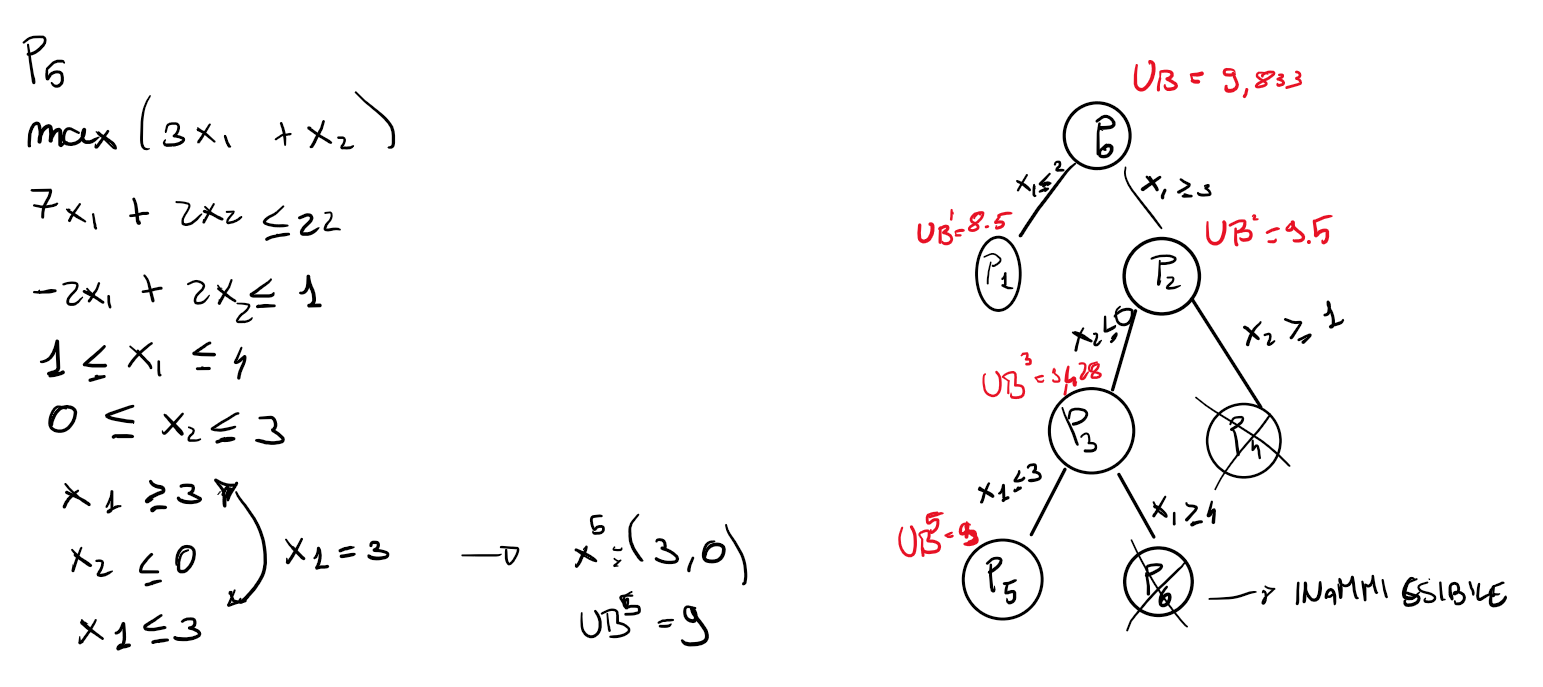
\includegraphics[width=1\linewidth]{Images/programmazione_lineare_continua/esempio_branch_bound/4.png}
\end{figure}
Concludiamo il problema notando che $P_1$ ha valore della funzione obiettivo inferiore a quello corrente, per cui non visitiamo più alcun nodo e concluderemo che la soluzione al problema di programmazione lineare intero è $x^5 = (3,0)$.
\section{Tecniche di Rilassamento}
L'operazione di bounding nel metodo del branch and bound viene generalmente effettuata attraverso il metodo del rilassamento lineare, tuttavia, esistono, in realtà, altre forme di rilassamento che adesso analizzeremo.
\subsection{Rilassamento per Eliminazione dei Vincoli}
Si consideri il problema di programmazione lineare intera $PLI_0$:
\[\min c^Tx \quad Ax \geq b \quad D x \geq d \quad x \in Z ^n\]
Supponiamo che i vincoli rendano difficile il problema siano i vincoli $Ax \geq b$, si effettua il rilassamento eliminando $Ax \geq b$ e risolvendo, invece:
\[\min c^Tx \quad Dx \geq d \quad x \in Z^n \] 
Risulterà che il valore ottimo $Z^n(PLI_1)$della funzione obiettivo di $PLI_1$ sarà un lower bound per il valore ottimo $Z^n(PLI)$ della funzione obiettivo di $PLI$. Cioè:
\[Z(PLI_1) \leq PLI\]
Quello che facciamo tramite il rilassamento lineare è un caso particolare di rilassamento per eliminazione dei vincoli.
\subsection{Rilassamento per Funzione Obiettivo Modificata}
Si consideri il problema $PLI_A$:
\[\min c^Tx \quad Ax \geq b \quad x \in Z ^n\]
E sia $d^Tx$ una funzione tale che:
\[d^Tx \leq c^Tx \quad \forall x: Ax \geq b \quad x\in Z^n\]
Si risolve il problema il problema $PLI_B$:
\[min d^Tx \quad Ax \geq b \quad x\in Z^n\]
E si avrà che  il valore ottimo della funzione obiettivo $PLI_B$ è $\leq$ del valore ottimo della funzione obiettivo di $PLI_A$: 
\[Z(PLI_B) \leq Z(PLI_A)\]
\subsection{Rilassamento Lagrangiano}
Questo metodo rappresenta un misto tra il rilassamento per eliminazione dei vincoli e rilassamento per funzione obiettivo modificata. Sia dato il problema PLI:
\[min c^Tx \quad Ax \geq b \quad Dx \geq d \quad x \in Z ^n\] 
E siano $Ax \geq b$ i vincoli difficili da trattare. Eliminiamo i vincoli $Ax \geq b$ e li inseriamo nella funzione obiettivo mediante un vettore $\lambda$. Si costruisce quindi il problema $PL_g$:
\[\min(c^Tx - \lambda (Ax-b)) \quad Dx \geq d \quad x\in Z^n \] 
Detto problema \textbf{lagrangiano}. Il vettore $\lambda$ è detto vettore dei moltiplicatori di Lagrange. Chiamiamo funzione Lagrangiana la funzione:
\[L(\lambda) = \min\{c^Tx - \lambda(Ax-b): Dx \geq d, x \in Z^n\}\]
Dunque:
\[L(\lambda) \leq Z(PLI)\]
E, anche in questo caso, avremo che la funzione obiettivo del problema lagrangiano rappresenta un lower bound per la funzione obiettivo del problema di programmazione intero. Inoltre, notiamo che variare di $\lambda$ si ottengono infiniti lower-bound per $PLI$. Il migliore si trova risolvendo il problema Lagrangiano duale:
\[max_\lambda L(\lambda) = max_\lambda (min_x {c^Tx - \lambda(Ax-b): Dx \geq d})\]
Se confrontiamo il rilassamento lagrangiano con il rilassamento lineare, si trova che:
\[L(\lambda*) \geq z(RL)\]
Dove $\lambda*$ è il valore ottimo del problema Lagrangiano duale e $Z(RL)$ è il valore ottimale della funzione obiettivo del rilassamento lineare di $PLI$. Un'altra cosa importante a cui fare riferimento per la corretta applicazione del metodo, è il fatto che $\lambda \geq 0$.
\section{Problema dello Zaino}
Sia E = {1, \dots, n} un insieme di oggetti e a ogni oggetto $i$ associamo un profitto $p_i$ e un peso
$w_i$ con $p_i, w_i \in N$. Sia C la capacità massima ($C \in N$). Vogliamo selezionare gli oggetti in
modo da massimizzare il profitto e rispettare la capacità dello zaino.
Si tratta di un problema di programmazione lineare intera di PLI. Introduciamo le variabili $x_i$ = {1 se l'oggetto è inserito nello zaino, 0 altrimenti} e vogliamo che:
\[\max \sum_i^n p_i x_i \quad vincoli: \sum_i^n w_i x_i \leq c \quad x_i \in \{0,1\}\]
Questo problema può essere risolto sia tramite metodologia greedy, sia tramite il metodo Branch and Bound.
\subsection{Metodo Greedy}
Si ordinano gli oggetti secondo un ordine opportuno. Si inseriscono gli oggetti nello zaino seguendo l'ordine. Se un oggetto non può essere inserito nello zaino, si scarta e si passa al successivo. Il metodo termina quando tutti gli oggetti sono visitati o si esaurisce la capacità dello zaino. I criteri per ordinare gli oggetti sono principalmente:
\begin{itemize}
    \item \textbf{Profitti crescenti:} si inseriscono prima oggetti di maggior valore.
    \item \textbf{Pesi non decrescenti:} si cercano di inserire quanti più oggetti possibili.
    \item \textbf{Rapporto valore/peso:} il rapporto valore peso rappresenta quanto si guadagna in rapporto al peso che si sta inserendo. Maggiore è questo valore, maggiore è il guadagno.
\end{itemize}
\subsection{Metodo Branch \& Bound}
Cerchiamo di descrivere le operazioni di Bounding e Branching in questo contesto:
\begin{itemize}
    \item \textbf{Bounding:} si effettua il rilassamento lineare, cioè risolviamo:
    \[\max \sum_i p_i x_i \quad \sum_i w_i x_i \quad x_i \in [0,1]\] 
    \item \textbf{Branching binario:} si effettua il branching e si vedrà come $x_i$ potrà valere o 0 oppure 1. Nel (RL) ordiniamo le variabili secondo il rapporto valore/peso decrescenti e risolviamo il RL effettuando gli inserimenti in ordine. Supponiamo di poter inserire per intero: 
    \[x_1=x_2=\dots = x_h = 1\]
    Per cui, la variabile $x_{h+1}$ non potrà essere inserita per intero ma solo in parte, per cui: 
    \[x_{h+1} = \frac{C - \sum_i^n x_i}{W_{h+1}}\]
    A questo punto avremo riempito lo zaino al massimo delle sue capacità, per cui tutti gli altri oggetti da $x_{h+2}$ a $x_n$ saranno $= 0$. Scegliamo come variabile di branch $x_{h+1}$ da cui nasceranno due problemi figli:\footnote{Un esempio è visibile su OneNote 17 Novembre}
    \begin{figure}[H]
        \centering
        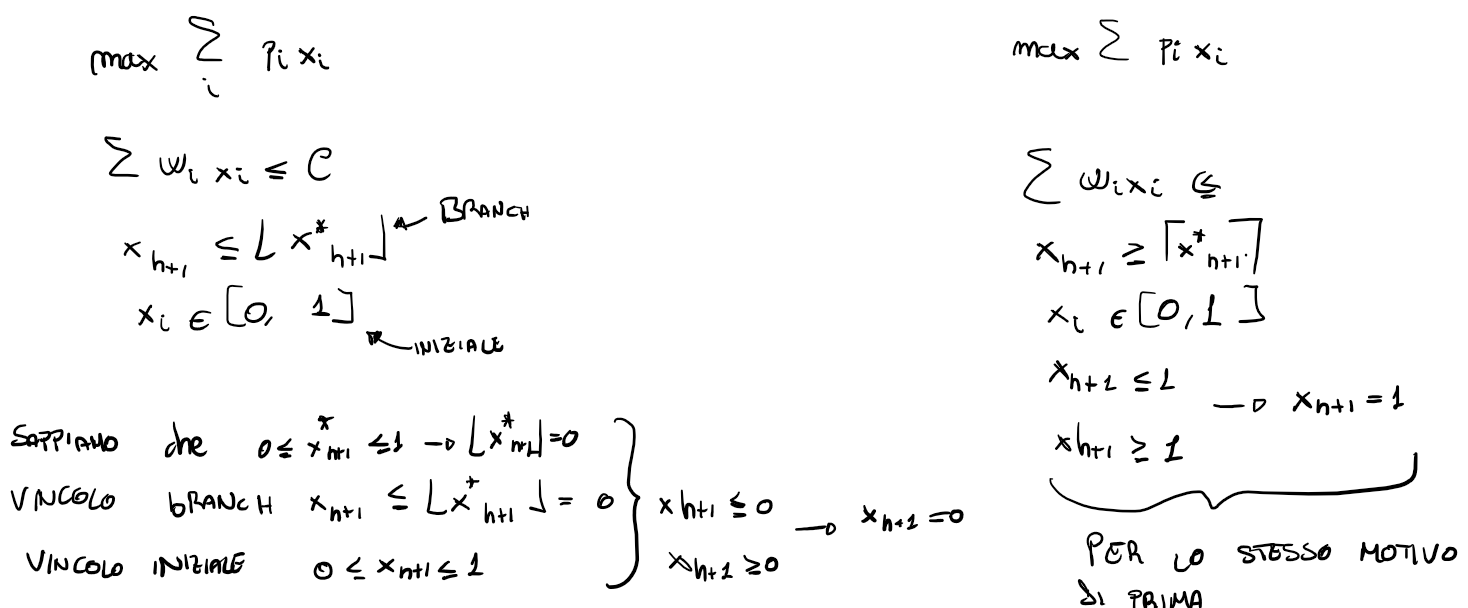
\includegraphics[width=1\linewidth]{Images/programmazione_lineare_continua/zaino/zaino_branch.png}
    \end{figure}
\end{itemize}
\section{Problemi di Assegnamento e Algoritmo Ungherese}
Un problema dell'assegnamento è n problema di programmazione lineare intera. Consideriamo due insiemi disgiunti con la stessa cardinalità. Siano
A e B: 
\[A \cap B = 0, \quad card(A) = card(B)\]

Assegniamo un costo $c_{ij}$ a ogni abbinamento di un elemento $i \in A$ con $j \in B$. Il problema dell'assegnamento vuole assegnare a ogni elemento di A univoco elemento di B e a ogni elemento di B un solo elemento di A minimizzando il costo e, nel caso in cui abbiamo cardinalità diverse, possiamo aggiungere elementi fittizi con costo nullo.

Avremo delle variabili $x_{ij}$ tale che il loro valore è 1 se $i \in A$ è accoppiato a $j \in B$ e 0 altrimenti. Il problema dell'assegnamento sarà dunque:
\[\min \sum_{i \in A} \sum_{j \in B} c_{ij} x_{ij}\]
I cui vincoli saranno:
\[\sum_{j \in B} x _{ij} = 1 \quad \forall i \in A \text{ ogni elemento di A si accoppia un solo elemento di B}\]

\[\sum_{i \in A} x _{ij} = 1 \quad \forall j \in B \text{ ogni elemento di B si accoppia un solo elemento di A}\] 
\[x_{ij} \in \{0,1\}\]

Per questo tipo di esercizi  matrice dei coefficienti è totalmente unimodulare. Quindi, il vincolo $x_{ij} \in \{0,1\}$ si può sostituire con il vincolo
$x_{ij} \in [0,1]$ dato che è un \textbf{problema ideale}.
\subsection{Algoritmo Ungherese}
Il metodo dell'algoritmo ungherese utilizza la matrice dei coefficienti ed effettua delle trasformazioni sulle righe e sulle colonne in modo tale da aumentare gli elementi nulli. Si effettuano delle riduzioni per righe e per colonne nel seguente modo:
\begin{itemize}
    \item \textbf{Riduzioni per righe}: a ogni riga si sottrae l'elemento $c_{ij} = c_{ij} - \min_j c_ij$
    \item \textbf{Riduzioni per colonna}: a ogni colonna si sottrae l'elemento minimo $c_{ij} = c_{ij} - \min_i c_ij$
\end{itemize}
Alla fine si avrà almeno uno zero in ogni riga e ogni colonna. Si cerca di creare l'assegnamento, accoppiando righe e colonne che hanno gli zeri in corrispondenza dell'incrocio. Se non si riescono ad abbinare tutte le righe e le colonne, si trasforma ancora la matrice. Si cerca il \textbf{ricoprimento minimo degli zeri} cioè i tagli minimi di righe e colonne che ricoprono tutti gli zeri. Per fare ciò, l'algoritmo utilizza il seguente metodo:
\begin{enumerate}
    \item Si etichettano le righe rimaste fuori dall'assegnamento.
    \item Si etichettano le colonne con zeri nelle righe etichettate.
    \item Si etichettano le righe accoppiate con le colonne etichettate.
    \item Si tagliano le righe non etichettate e le colonne etichettate.
    \item Infine, si cerca l'elemento minimo tra quelli non barrati e si sottrae agli elementi non barrati e si somma agli elementi a incrocio tra righe e colonne per poi scegliere l'assegnamento.
\end{enumerate}

È importante sottolineare che per indicare i costi dell'assegnazione, serve guardare la matrice iniziale dei costi. Un esempio:
\begin{figure}[H]
    \centering
    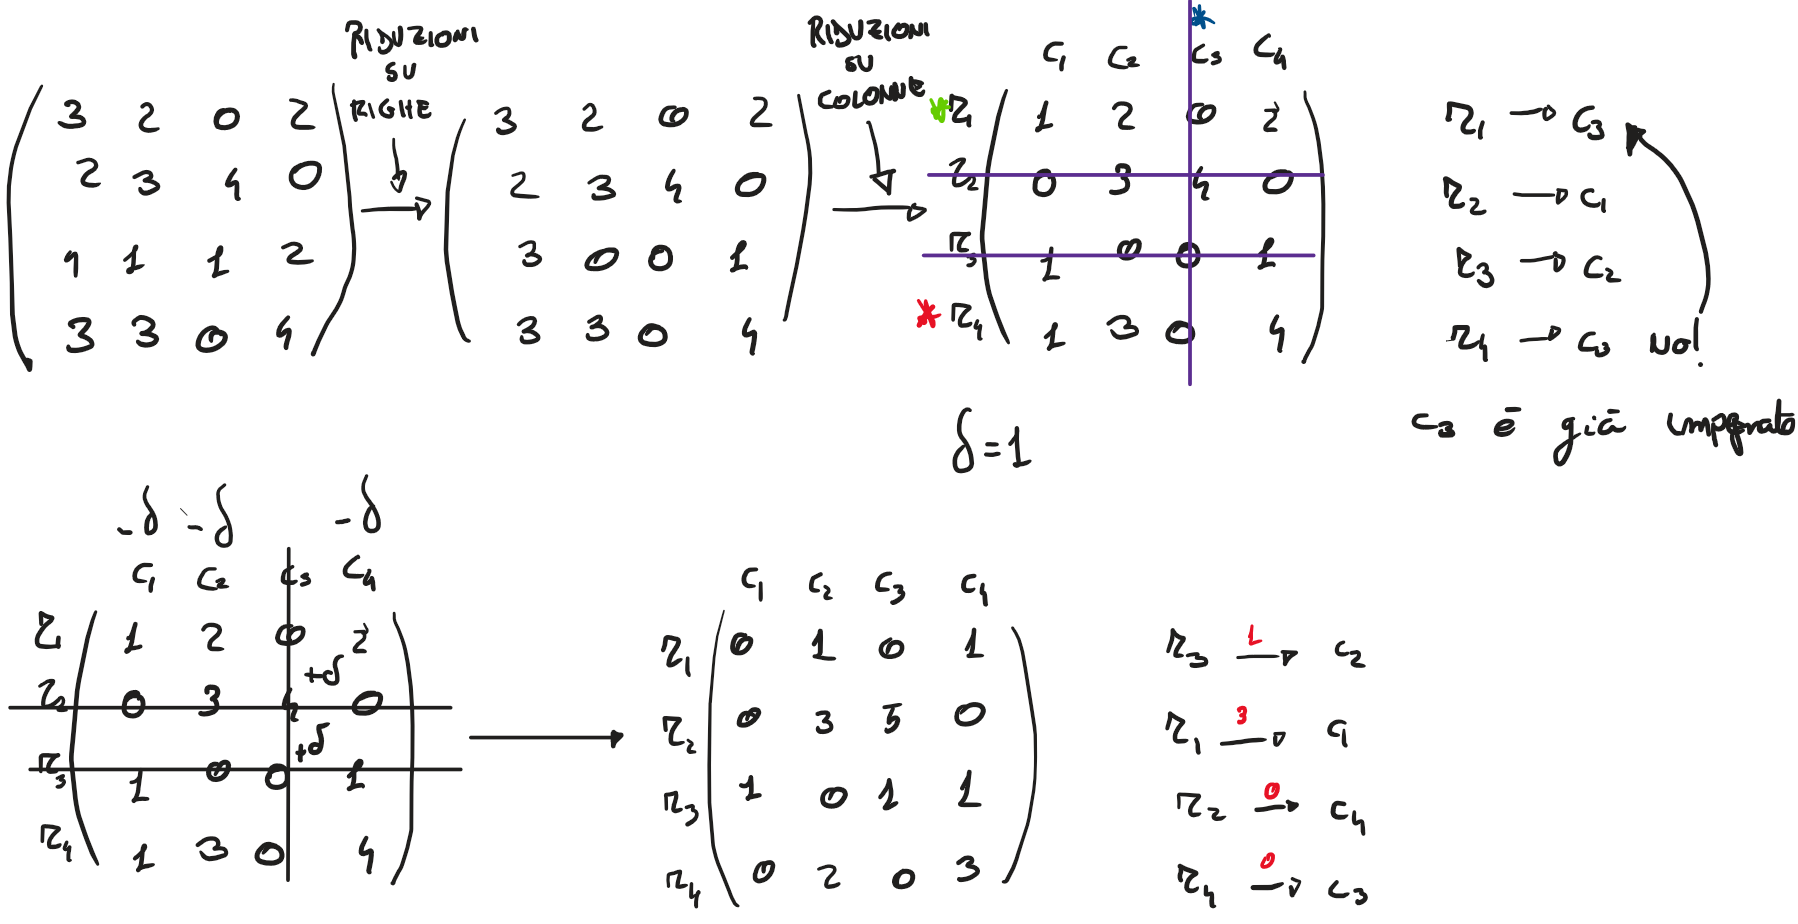
\includegraphics[width=1\linewidth]{Images/programmazione_lineare_continua/algoritmo_ungherese_esempio.png}
\end{figure}

\section{Problema del Commesso Viaggiatore (TSP)}
Il problema del TSP si può formulare su un grafo orientato $G=(N, A)$ dove a ogni arco $(i, j)$ si associa un costo $c_j$. Il problema consiste nel determinare un ciclo Hamiltoniano, cioè che tocca ogni nodo una sola volta, e che questo sia di costo minimo.

Si può considerare anche un problema del TSP su un grafo non orientato attribuendo un costo a ogni spigolo\footnote{Per spigolo si intende un arco in un grafo non orientato} del grafo. Nello specifico, in questa trattazione parleremo del problema TSP asimmetrico\footnote{Il caso simmetrico è quello con grafi non orientati per cui da l'arco $(A,B)$ ha lo stesso costo dell'arco $(B,A)$} per grafi orientati.

Questo problema sarà formulato nel seguente modo:
Sia $G= (N, A)$ e sia che a ogni arco $(i, j)$ assegniamo un costo $c_{ij}$, introduciamo la seguente variabile:
\[
x = 
\begin{cases} 
   1 & \text{se } x_{ij} \text{ è parte del ciclo Hamiltoniano} \\
   0 & \text{altrimenti}
\end{cases}
\]
Il problema del TSP è un problema di programmazione lineare intera 0,1:
\[\min\sum_{(i,j) \in A} c_{i,j} x_{i,j}\]
Con vincoli:
\[\sum_{i \in N; (i,v) \in A} x_{i,v} = 1 \quad \forall v \in N \quad \text{In ogni nodo entra un solo arco}\]
\[\sum_{j \in N; (v, j) \in A} x_{v, j} = 1 \quad \forall v \in N \quad \text{Da ogni nodo esce un solo arco}\]
Un ulteriore vincolo da considerare è che  $\forall S \subset N, 2 \leq |S| \leq |N| -1$\footnote{NB: questo N-1 serve a non eliminare tutti i
cicli del grafo, altrimenti non potrebbe esserci ciclo}. Ossia, non devono esservi sottocicli nel ciclo considerato, in formule: 
\[\sum_{i, j \in S; (i,j) \in A} x_ij \leq |S| -1 \]

Vediamo adesso come risolvere questo tipo di problemi. Come per lo zaino, considereremo un metodo greedy e un metodo esatto basato sul branch and bound. Una precisazione necessaria prima di continuare con il metodo è che questo prevede che il grafo sia completo, se così non è, si aggiungono gli archi mancanti con costo $\infty$ in maniera tale da scoraggiarne l'uso.


\subsection{Metodo Greedy}
Partendo dal primo nodo, si seleziona il nodo che ha distanza minima da esso. Così facendo, si costruisce un ciclo hamiltoniano che, tuttavia, potrebbe non essere il ciclo hamiltoniano ottimo. Vediamone un esempio:
\begin{figure}[H]
    \centering
    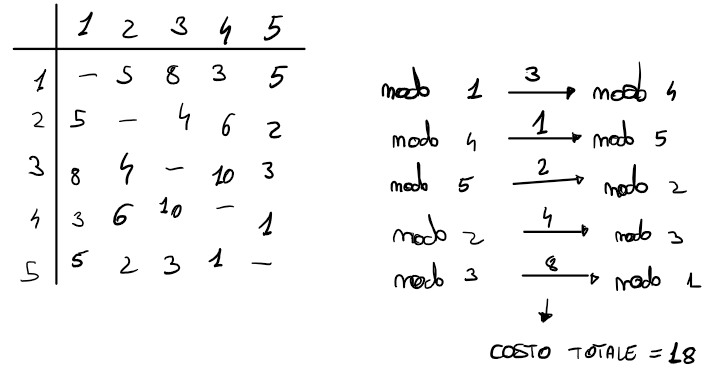
\includegraphics[width=0.5\linewidth]{Images/programmazione_lineare_continua/tsp/esempio_greedy.png}
\end{figure}

\subsection{Metodo Branch \& Bound}
Per capire come effettuare il metodo branch and bound, abbiamo innanzitutto la necessità di capire come effettuare queste due operazioni:
\begin{itemize}
    \item \textbf{Bounding}: Si andrà a risolvere il rilassamento per eliminazione del vincolo sui sottocicli, per cui, passeremo al seguente problema:
    \[
        \begin{cases}
        \min \sum_{i=1}^n \sum_{j=1}^n c_{ij}x_{ij} \\
        \sum_{\substack{i=1 \\ i \neq j}}^n x_{ij} = 1, \quad j \in N \\
        \sum_{\substack{j=1 \\ j \neq i}}^n x_{ij} = 1, \quad i \in N \\
        x_{ij} \in \{0, 1\}, \quad \forall i, j \in \{1, \dots, n\}, i \neq j.
        \end{cases}
    \]
    Questo problema è equivalente al problema dell'assegnamento dove si duplica l'insieme N dei nodi del grafo per ottenere i due insiemi dei nodi da accoppiare che abbiano la stessa cardinalità. L'insieme N si duplica e pertanto $N_1 = N$ e $N_2 = N$, si ottiene il problema:
    \[
        \begin{cases}
            \min \sum_{i \in N_1}^n \sum_{j \in N_2} c_{ij}x_{ij} \\
            \sum_{i \in N_1}^n x_{ij} = 1, \quad j \in N_2 \\
            \sum_{j \in N_2}^n x_{ij} = 1, \quad i \in N_1 \\
            x_{ij} \in \{0, 1\}, \quad \forall i, j \in \{1, \dots, n\}.
        \end{cases}
    \]
    A questo punto, se la soluzione dell'assegnamento è un ciclo hamiltoniano, allora è soluzione del TSP. Se la soluzione non è un ciclo Hamiltoniano, allora vuol dire che conterrà dei sottocicli. Si sfrutteranno quindi i sottocicli per effettuare l'operazione di Branch.
    \item \textbf{Branching:} Per eliminare il sottociclo si elimina uno degli archi che lo compone. In generale, per eliminare un arco $(i, j)$, si impone che $x_{ij} = 0$ e nella matrice dei costi si pone $c_{ij} = \inf$. Data la soluzione dell'assegnamento, si seleziona il sottociclo di cardinalità minima, ad esempio, se si trovano i cicli $ 1\rightarrow 2 \rightarrow 1$ e $3\rightarrow 4\rightarrow 5 \rightarrow 3$, si sceglierà $1\rightarrow 2 \rightarrow 1$ formato dagli archi (1,2) e (2,1). \footnote{Nel caso di più cicli con la stessa cardinalità, se ne sceglie uno casuale} A questo punto, una volta scelto il ciclo $(1 \rightarrow 2 \rightarrow 1)$, si genereranno due figli in maniera tale che in un uno non ci sia l'arco $(1,2)$ e nell'altro non ci sia $(2,1)$. Per questioni legate al funzionamento del metodo, nel secondo caso, inseriremo il nodo precedente come scelta obbligata.  
    \begin{figure}[H]
        \centering
        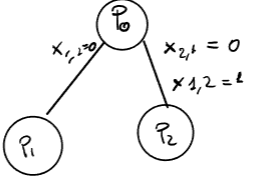
\includegraphics[width=0.35\linewidth]{Images/programmazione_lineare_continua/tsp/esempio_branch.png}
    \end{figure}
    Più in generale, dato il sottociclo 
    \[c' = { (i_1, j_1), (i_2, j_2), \dots, (i_k, j_k)}\]
    Nascono $k$ nodi figli tale che:
    \begin{itemize}
        \item Nel primo problema si pone $x_{i_1, j_1} = 0$
        \item Nel secondo problema si pone $x{i_2,j_2} = 0, x_{i_1, j_1} = 1$
        \item Nel terzo problema $x_{i_3, j_3} = 0, x_{i_1, j_1} = 1, x{i_2,j_2} = 1$
        \item E così via, nell'ultimo $x_{i_k, j_k} = 0$ e tutti gli altri $x_{i,j} = 1$.
    \end{itemize}
\end{itemize}
Vediamo un esempio:
\begin{figure}[H]
    \centering
    
\includegraphics[width=1\linewidth]{Images/programmazione_lineare_continua/tsp/esempio_branch_bound/1.png}
\end{figure}
\begin{figure}[H]
    \centering
    
\includegraphics[width=1\linewidth]{Images/programmazione_lineare_continua/tsp/esempio_branch_bound/2.png}
\end{figure}
\begin{figure}[H]
    \centering
    
\includegraphics[width=1\linewidth]{Images/programmazione_lineare_continua/tsp/esempio_branch_bound/3.png}
\end{figure}
\begin{figure}[H]
    \centering
    
\includegraphics[width=1\linewidth]{Images/programmazione_lineare_continua/tsp/esempio_branch_bound/4.png}
\end{figure}